\chapter{\IfLanguageName{dutch}{Stand van zaken}{State of the art}}%
\label{ch:stand-van-zaken}

\nocite{Paper}

In dit hoofdstuk wordt eerst bekeken wat een API juist is. De precieze werking van REST alsook van gRPC worden daarna grondig onderzocht met extra aandacht voor
eventuele aspecten die de performantie kunnen beïnvloeden. Tot slot worden beide technologie\"en ook met elkaar vergeleken.

\section{API}

Een application programming interface, vaker API genoemd, is een connectie tussen computers of applicaties.
Een API-specificatie verwijst dan weer naar een standaard die beschrijft hoe een dergelijke interface of connectie moet werken.
Van een applicatie die deze standaard volgt, wordt gezegd dat ze een API blootstelt. API kan verwijzen naar de standaard zelf of naar de applicatie die deze implementeert.
Zeer vaak wordt, wanneer naar een API wordt verwezen, een web API bedoeld. Een web API bewerkstelligt de communicatie, die via het internet verloopt, tussen applicaties.\\

API's worden ontzettend veel gebruikt waardoor ze ook zeer belangrijk zijn. Elke website, elke browser, maar ook nagenoeg elk apparaat dat met internet verbonden is,
de zogenaamde smart devices, maakt er gebruik van. De evolutie in de technologische ontwikkeling is van die aard dat er steeds meer apparaten verbonden zijn met elkaar
en dat deze apparaten ook steeds vaker, en tevens grotere, datasets versturen. Aan de hand van de API's zijn consumenten in staat deze apparaten aan te sturen en te monitoren
en daarnaast zorgen ze voor een massa aan data die direct bruikbaar is of het potentieel heeft om bruikbaar te worden. Data die, vanuit het standpunt van de producenten, niet mag verloren gaan.\\

Het wijdverspreide gebruik van API's, de constante toename van dat gebruik, en zeker ook de toename van de grootte van de data die wordt verzonden, toont
direct aan dat performantie een zeer belangrijk punt is. Elke softwareontwikkelaar of -architect dient hier rekening mee te houden, en moet het ontwerp van de
applicatie alsook de keuze voor bepaalde technologie\"en afstemmen op de noden van de applicatie en haar gebruikers.\newline
~\autocite{cleo}\\

REST en RPC zijn beiden API's en meer specifiek web API's in die zin dat ze specificaties zijn die aangeven hoe een connectie tussen twee systemen kan geïmplementeerd worden.
gRPC daarentegen is een implementatie van Google van de RPC specificatie.\\

Buiten REST en gRPC zijn er nog verschillende vari\"eteiten van web API's welke niet verder aan bod zullen komen in deze scriptie, maar die toch interessant zijn om
te vermelden en kort te vergelijken met de twee die het onderwerp zijn van dit onderzoek.


\paragraph{SOAP}
Simple Objects Access Protocol ofwel kort SOAP is een web communicatie protocol ontwikkeld voor Microsoft in 1998. Het wordt op vandaag het meeste gebruikt om
web services aan te bieden via HTTP of HTTPS(HTTP over TLS of SSL) maar kan ook gebruikt worden bij bv. FTP en SMTP.\newline
Bij SOAP wordt data, in XML formaat, steeds via een standaard XML schema (XSL) ge\"encodeerd. Zo worden berichten, requests en responses, als volgt gestructureerd:
Een <soap:Envelope> is het hoofdelement en kan drie sub-elementen bevatten nl. <soap:Header>, <soap:Body> en <soap:Fault>. De Header is optioneel maar moet
als eerste voorkomen binnen de Envelope. Dit element geeft eventuele extra informatie m.b.t. het bericht en kan bv. de authenticatie gegevens bevatten. Het Body element
is noodzakelijk en bevat de effectieve data van het bericht, tevens in XML formaat. Het niet verplichte Fault element bevat ten slotte gegevens over eventuele errors.\newline
SOAP zelf legt standaard enkel deze basis-structuur op. Wat er verder in de Header of Body elementen wordt geplaatst, wordt niet bepaald. SOAP werd, door deze lacune, na haar
uitgave uitgebreid met een veelvoud van protocollen die in meer detail de werking specifi\"eren. Deze gaan over verschillende onderwerpen zoals beveiliging, transactiebeheer,
metadata,\ldots. WS-Atomic Transaction is een voorbeeld waarmee aan de ACID (Atomair, Consisitent, Ge\"{\i}soleerd en Duurzaam) regels kan voldaan worden.
Met behulp van Web Service Description Language of kort WSDL kan, in XML formaat, een schema gedefinieerd worden welke dienen als richtlijn om met een web service te
communiceren. Aan de hand van dit schema kan code bij de client gegenereerd worden. SOAP staat zowel stateful als stateless communicatie toe, waar de server respectievelijk
informatie over de client gaat bijhouden of juist niet.\newline
Enkele nadelen van SOAP zijn de grotere bestandsgrootte van XML waar men bij SOAP niet rond kan, het feit dat het gebaseerd is op een groot aantal protocollen waarbij
de verschillende nodige protocollen begrijpen voor een stevige leercurve kan zorgen en tot slot het strikte contract tussen server en client weinig flexibiliteit geeft
waardoor een simpele aanpassing een vervelend en omvangrijk proces kan worden.\newline
~\autocite{soap,redhatapissoaprestgraphqlgrpc}\\

\paragraph{GraphQL}
GraphQL is een technologie die eerst werd ontwikkeld door Facebook maar werd intussen open-source gemaakt. Bij GraphQL wordt de communicatie gestart doordat de
client een HTTP POST request verstuurd naar de server. In de body van die request zit een GraphQL query of mutation die aangeeft welke data respectievelijk wordt
opgevraagd of gewijzigd. De inhoud van deze query moet in eerste instantie voldoen aan specificaties van GraphQL zelf, maar daarnaast ook aan het schema dat gedefinieerd
wordt door de server. In de server applicatie wordt een GraphQL schema opgesteld waarin de beschikbare objecten, in de vorm van types, omschreven worden. De mogelijke
queries en mutations worden ook hier opgelijst. Door de data in dit GraphQL formaat weer te geven is de representatie ervan, zoals de naam al zegt, in een graph.
De types zijn nodes die via edges, al dan niet bidirectioneel, aan elkaar verbonden zijn. GraphQL is zeer flexibel naar de client toe om te bepalen welke data deze opgevraagt.
De client kan starten vanop een gedefinieerd query of mutation entrypoint en zo aangeven welke data hij effectief wenst terug te krijgen, tot gerelateerde nodes toe.
Hij kan, indien dit via het schema beschikbaar werd gemaakt, eventueel zelfs extra input meegeven om geconnecteerde nodes aan te spreken. Vooral voor frontend ontwikkelaars
biedt dit een groot voordeel aangezien zij specifiek enkel de data kunnen opvragen die ze op het scherm zullen weergeven, niet meer, niet minder, en waarschijnlijk slechts met \'e\'en oproep.
Naast queries en mutations, welke beiden een synchroon verloop kennen, biedt GraphQL nog een derde mogelijkheid aan nl. subscriptions, dat asynchroon werkt.
Via een subscription kan een client zich inschrijven om bepaalde berichten vanuit de server te ontvangen. Zo kan de server de client bijvoorbeeld een bericht sturen als
een bepaalde gebeurtenis zich heeft voorgedaan. Subscriptions werken aan de hand van WebSockets en dus niet meer via het HTTP protocol. Het implementeren van subscriptions
kan blijkbaar wel wat meer moeilijkheden met zich meebrengen.\newline
~\autocite{graphql,redhatapissoaprestgraphqlgrpc,graphqlfrontend,graphqlsubscriptions}\\

Om de twee juist beschreven API's goed te kunnen plaatsen qua gebruik en belang wordt hier wat voorgelopen op de verdere uitleg en alvast een overzicht getoond van de evolutie van de
stack overflow trends sinds 2008 met betrekking tot de tags SOAP en GraphQL. Later meer over REST vs gRPC. Met betrekking tot SOAP en GraphQL is alvast zeer duidelijk dat SOAP eerder
aan populariteit aan het inboeten is, eventueel met juist een kleine opleving sinds 2022. GraphQL daarentegen is sinds einde 2015 fors gestegen naar hetzelfde niveau dat SOAP had
op haar hoogtepunt op de grafiek in figuur~\ref{fig:stackoverflowSOAPGraphQL} nl. in 2008. GraphQL lijkt haar stijging sinds 2020 slechts zeer licht verder te zetten.
\begin{figure}[ht]
    \centering
    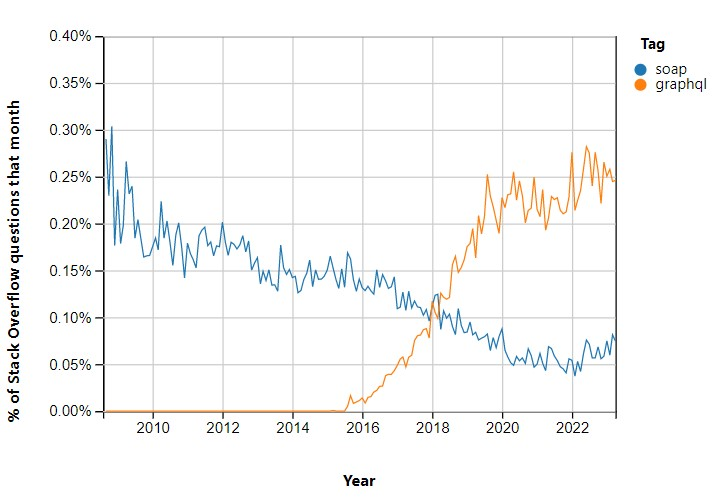
\includegraphics[width=1.0\linewidth]{stackoverflowSOAPGraphQL}
    \caption{Percentage Stack Overflow vragen per maand voor SOAP en GraphQL,\newline
    https://insights.stackoverflow.com/trends?tags=soap\%2Cgraphql}
    \label{fig:stackoverflowSOAPGraphQL}
\end{figure}\\
\nocite{stackoverflowSOAPGraphQL}


\section{REST}

Representational State Transfer, vaker benoemd door middel van het acronym REST, is een type van web API. Deze technologie wordt zeer vaak gebruikt om webservices te bouwen.
Dit zijn applicaties die diensten of data als web resources aanbieden. Door middel van een REST API kan de client om deze resources vragen zonder verder
begrip van de interne werking van de provider. De server reageert dan door een response te versturen met een status code en met de resource in JavaScript object Notation (JSON),
Extensible Markup Language (XML) of andere tekstindelingen. Een web resource is eigenlijk alles waarmee een client op het web kan communiceren.
Het kan betrekking hebben op een bestand, afbeelding, HTML of video. Een resource kan ook een service zijn zoals Google Maps of een financi\"ele dienst.
De API-ontwikkelaars moeten de beslissing maken welke resources ze ondersteunen voor de response.
De API moet de mogelijkheid hebben om de response op te maken op basis van de behoefte van de client.\newline
~\autocite{uptrends,guru99-webservices}\\

Opdat een API als RESTfull kan worden beschouwd moet het aan enkele kenmerken voldoen.\newline
Ten eerste dient het, voor de communicatie, op zijn minst gebruik te maken van het HTTP 1.1 protocol. Het protocol, dat zich in de applicatie laag situeert,
bepaalt dat de client een request, met tekst als vorm, verstuurt naar de server waarop die de gevraagde gegevens terugzendt.
HTTP specificeert verschillende soorten requests methods waaronder GET, POST, PUT en DELETE. Een REST API kan van al deze methods gebruik maken en zal dat
hoogstwaarschijnlijk ook doen. HTTP 1.1 houdt een TCP-connectie open tot er uitdrukkelijk opdracht gegeven wordt om deze te sluiten.
Dit geeft een enorme performantie winst t.o.v. HTTP 1.0. Het nadeel van deze uitdrukkelijke opdracht is dat een wachtende request alle achterliggende requests kan blokkeren.
Extra TCP-connecties kunnen hier een oplossing bieden, deze zijn echter ook gelimiteerd.\newline
~\autocite{w3Protocol}\\
Als tweede kenmerk moet een REST API stateless zijn. Dit houdt in dat er geen informatie zal worden opgeslagen tussen requests door.
De API zal de verbinding tussen server en client verbreken nadat de server een resource in de vorm van een response heeft doorgezonden aan de client.
De API behandelt zo elke request los van een eventuele vorige request. Dit vermindert de hoeveelheid geheugen die een server nodig heeft en verhoogt de
kans op een succesvoller antwoord omdat de server geen extra stappen moet nemen om oude data op te zoeken.\newline
Het derde kenmerk voorziet erin dat de verstuurde data cacheable moet zijn. De client weet namelijk a.d.h.v het type van REST request,
meer specifiek de request method, dat hij verzonden heeft wat voor antwoord hij kan verwachten.\newline
De vierde eigenschap bestaat uit de verplichting een uniforme interface tussen componenten te voorzien zodat data kan verzonden worden in een standaard vorm.\newline
Het vijfde kenmerk specificeert dat het niet noodzakelijk mag zijn dat de client kennis heeft van de verdere werking van de server(s) buiten de vorm van de communicatie zelf.\newline
Tot slot laat het zesde, en enige optionele, kenmerk toe om executeerbare code te verzenden indien zo verzocht wordt door de client.\newline
~\autocite{redhat}\\

REST API's zijn flexibel. Ze kunnen requests van verschillende types aan alsook kunnen ze data versturen in verschillende formaten.
Webapplicaties groeien aangezien er telkens meer resources worden toegevoegd. Een REST API zal deze toenemende hoeveelheid van vari\"erende requests snel kunnen behandelen.\\

Een REST API spitst zich steeds toe op het domein dat het als resource zal aanbieden.
Dankzij deze focus en de uniforme manier van werken is het voor een client duidelijk welke functionaliteiten er kunnen worden aangeroepen en hoe dat te doen.\newline
~\autocite{jscrambler,hubspot,HTTP1.1vsHTTP2}\\

Afhankelijk van de taal waarin, de tussen server en client, verstuurde data zich bevindt, alsook de programmeertaal van beide applicaties,
zal er bij zowel de client als de server een serialisatieproces moeten plaatsvinden. Er zijn verschillende libraries die de serialisatie kunnnen verzorgen,
zo kan er bij Java gebruik gemaakt worden van bv. Jackson~\parencite{jackson} \newline
Bij de client zal gebruik moeten gemaakt worden van documentatie van de server applicatie of door de endpoints manueel aan te roepen
en zo op basis van de response de mapping voor het serialisatieproces op te maken. Het schrijven van de documentatie,
het cre\"eren van de code in de client om het REST API van de server aan te roepen en zelfs de code in de server kan automatisch gegenereerd worden dankzij
handige hulpmiddelen zoals bv. Swagger~\parencite{swagger}.\\

Tijdens de levensduur van een API is het bijna onvermijdelijk dat er aanpassingen gebeuren. Sommige van deze aanpassingen, zoals het toevoegen van een extra veld aan een object,
hebben geen invloed op eventuele clients en worden daarmee non-breaking changes genoemd. Andere aanpassingen, de zogenaamde breaking changes, hebben als gevolg dat er
fouten kunnen optreden bij clients. Zo kan het verwijderen van een veld uit een object plots een error veroorzaken bij
een client die het API aanroept en verwacht dat dit veld aanwezig is. In REST API's wordt, wanneer een breaking change ge\"{\i}mplementeerd wordt,
meestal gewerkt met een versie verhogen, ook version bump genoemd. De client moet dan bij elke request aangeven welke versie er wordt aangeroepen.
Dit kan door een aparte url per versie, door het versienummer mee te geven in een specifieke request header of door de versie aan de Accept header toe te voegen.
Deze verschillende versies kunnen in dezelfde applicatie ondersteund worden. Een andere optie is verschillende versies van de applicatie deployen.\newline
~\autocite{restversion}\\

Wanneer er via een REST API een grote dataset beschikbaar wordt gesteld, wordt het aanzien als best practice om een soort van paginatie te voorzien. Door paginatie te
implementeren kan de grote dataset in kleinere delen worden opgevraagd. Hierdoor zal het systeem minder makkelijk overbelast worden doordat \'e\'en proces lang blijft
hangen wanneer het een request aan het verwerken is. Wanneer de dataset daarenboven wordt gebruikt door een applicatie die een user interface voorziet zal het
niet wenselijk zijn om een te grote dataset in één keer weer te geven. Dit is immers niet overzichtelijk voor een menselijke gebruiker.
Deze gebruiker zal ook wensen dat de data in enkele seconden wordt weergegeven. Kleinere datasets zullen ook een positief effect hebben op de laadtijd.
Het netwerkverkeer van een applicatie wordt dankzij paginatie ook meer gericht gebruikt voor wat effectief nodig is. Het is ook aangewezen dat een REST API een
default paginagrootte implementeer voor wanneer deze parameter door de client niet wordt meegegeven. Daarenboven is het beperken van de maximum paginagrootte die
kan opgevraagd worden ook een goed idee.\newline
Praktisch komt paginatie bij een REST API er vaak op neer dat de client een paginanummer en een paginagrootte meegeeft wanneer er een dataset opgevraagd wordt.
Deze paginanummer en paginagrootte kan bij een GET request best in de url als query parameters meegegeven worden en bij een POST request eventueel in de request body.
De server zal dan de dataset, die wordt verzonden, beperken door de items voor de gevraagde pagina over te slaan en alle items na de opgegeven grootte te laten vallen.
Als bijkomende informatie zal de server de dataset aanvullen met pagina-informatie. Hier zal het paginanummer en de paginagrootte steeds toe behoren maar eventueel
ook aangevuld met het totaal aantal items en het totaal aantal pagina's van die grootte.
Stel dat via een REST API een lijst van boeken kan opgevraagd worden via een GET endpoint met page en pageSize query parameters. De request voor de eerste pagina
van 3 boeken zou er dan bijvoorbeeld zo kunnen uitzien:\newline
https://www.hogent.be/boeken?page=0\&pageSize=3
Het antwoord van de server, in JSON formaat, zou dan als volgt kunnen zijn:\newline
\{
''page'': 0,
''pageSize'': 3,
''totalCount'': 50,
''totalPages'': 17,
''results'': [\ldots]
\}\newline
~\autocite{paging}\\
~\autocite{wachtenLaadtijd}\\


\section{gRPC}

Een RPC API stelt een client in staat om op afstand een serverfunctie aan te roepen, zonder dat de client zich verder bewust hoeft te zijn van de interne werking
van de server of de implementatie van de functie.
RPC maakte in het verleden, net zoals REST, gebruik van het HTTP-protocol. De XML-RPC alsook de JSON-RPC implementaties zijn hier voorbeelden van.
Zij maken gebruik van de HTTP request methods GET en POST. De eerste voor het ophalen van data en de tweede voor alle andere functies.\\

De functies van een RPC API kunnen specifiek gericht zijn op de functionaliteit die ze implementeren en daarmee potentieel ook lichtgewicht zijn.
De client moet enkel de naam van de functie specifici\"eren en de vereiste data meegegeven. De response zal ook enkel de data bevatten die door de server nodig wordt geacht.
Wanneer de functies zodanig toegespitst zijn op een functionaliteit wordt er aan de consumer inzicht gegeven over de interne werking van de server,
alsook dient de client vaak kennis te hebben over die interne werking om de functies te kunnen gebruiken.\newline
~\autocite{altexsoft}\\

Google Remote Procedure Calls (gRPC) is de implementatie van Google van het RPC API.\\
Een eerste groot verschil tussen RPC en de implementatie van Google is dat gRPC gebruikmaakt van het HTTP 2-transportprotocol.
HTTP 2 werd in 2015 uitgebracht. De doelstellingen bij het ontwikkelen van deze nieuwe versie van het protocol waren vooral toegespitst op performantie.
Hierbij werden enkele nieuwe functies en kenmerken ontwikkeld. Request multiplexing laat toe om requests simultaan te laten gebeuren.
Dankzij Request prioritization kan een prioriteit gegeven worden aan requests. Requests en responses worden nu automatisch gecomprimeerd in tegenstelling tot op
uitdrukkelijk verzoek. De mogelijkheid om de verbinding te resetten werd toegevoegd. Daarenboven kan de server ook proactief resources verzenden naar de
cache van clients via de zgn. server push functie. En tot slot is HTTP 2 een binair protocol t.o.v. het op gewone tekst gebaseerde HTTP 1.1 protocol.\newline
~\autocite{baeldung}\\

Het verplicht gebruik van HTTP 2 komt echter ook met het nadeel dat gRPC hierdoor niet ondersteund wordt door de hedendaagse browsers. Javascript heeft geen
volledige controle over HTTP 2 waardoor er bepaalde HTTP 2 functionaliteit, die nodig is voor gRPC, niet beschikbaar is voor browsers die Javascript gebruiken.
Voor gRPC moeten er bijvoorbeeld trailing headers blootgesteld worden welke door browser steeds verborgen worden. Een oplossing hiervoor is het gebruik van een proxy welke
door middel van een normale HTTP request communiceert met de browser en dan de request via gRPC naar de server doorgeeft.\newline
~\autocite{altexsoftgrpc}\\
~\autocite{yukutakahashi}\\

Het HTTP 2 protocol verplicht het gebruik van encryptie zoals TLS niet, ondanks hevige discussie in de werkgroep. Het protocol legt wel enige verplichtingen op,
onder meer met betrekking tot het versienummer, wanneer er toch van encryptie of TLS gebruik wordt gemaakt. TLS staat voor Transport Layer Security en is een protocol
dat het encrypteren van data, die tussen applicaties over het internet verzonden wordt, specifieert. Door het dataverkeer te encrypteren zijn de verzender en ontvanger zeker dat
de berichten enkel door hen gelezen kunnen worden alsook dat deze berichten authentiek zijn en van hen afkomstig zijn. TLS wordt voor veel verschillende soorten van internet communicatie gebruikt.
Ondanks het niet verplichten van encryptie in het HTTP 2 protocol wordt TLS in de praktijk toch verplicht wanneer er gebruikgemaakt wordt van HTTP 2.
Gezien gRPC steeds via het HTTP 2 protocol gaat, zal TLS dan eventueel ook moeten voorzien worden bij gRPC API's. Het gebruik van TLS bij gRPC wordt daarenboven aangeraden.
HTTP 2 wordt door de meeste browsers wel gesupporteerd, maar steeds in combinatie met TLS. Het is niet omdat een browser het HTTP 2 protocol aanvaardt dat daarmee gRPC reeds
gesupporteerd wordt.\newline
TLS heeft een impact op de performantie. Bij TLS moet er een onderhandeling gevoerd worden met wat heen en weer communicatie. Bij het HTTP 2 protocol blijft het
negatieve effect, van deze onderhandeling, op de performantie lager dan bij HTTP 1.1., mede dankzij het gebruik van multiplexing.
Een server moet een SSL/TLS certificaat hebben om deze encryptie te kunnen gebruiken. Dit certificaat zal in eerste instantie toelaten om de identiteit van het systeem
waarmee een connectie tot stand gebracht wordt te achterhalen en daarna helpen de communicatie over de connectie te encrypteren. Er bestaan zelf gesigneerde certificaten
en CA certificaten gecre\"eerd en gesigneerd door een Certificate Authority. Een self signed certificate wordt normaal alleen geaccepteerd als dit certificaat of de
partij die het getekend heeft gekend is door de consumerende applicatie en dus bijna exclusief voor intern gebruik. CA certificates kunnen geaccepteerd worden indien de
CA zelf vertrouwd wordt door de applicatie.\newline
TLS gaat met deze certificaten symmetrische en asymmetrische encryptie toepassen. Via asymmetrische encryptie wordt een beveiligde sessie tussen server en client tot
stand gebracht waarna de uitgewisselde data via symmetrische encryptie wordt beveiligd. Het proces verloopt als volgt.
\begin{itemize}
    \item De client contacteert de server via HTTPS.
    \item De server verstuurt zijn certificaat en publieke sleutel.
    \item De client verifieert het certificaat met een vertrouwde CA of controleert of het certificaat zelf vertrouwd wordt.
    \item Client en server onderhandelen over de te gebruiken encryptie.
    \item De client encrypteert een sessie sleutel, specifiek voor de sessie, door middel van de publieke sleutel en verstuurt deze naar de server.
    \item De server gebruikt zijn private sleutel om de sessie sleutel te decrypteren en de sessie wordt vastgesteld.
    \item Client en server gebruiken nu de sessie sleutel om de communicatie te encrypteren en decrypteren.
\end{itemize}
~\autocite{githubhttp2,sslcomhttp2tls,browserhttp2support,tlsBasics,grpctls,http11vshttp2,tlsperformance,sslcertificate,sslhandshake}\\


gRPC gebruikt geen JSON, XML, of zelfs enig ander tekstformaat, maar protocol buffers, ook protobuf genoemd. Protobuf is zodanig geformatteerd dat het niet leesbaar is
voor het menselijk oog. Berichten worden verkleind tot een binair formaat waardoor de snelheid van data transacties hoger zou liggen. gRPC heeft een ingebouwde
protoc-compiler voor het genereren van API-aanroepen en kan zo makkelijk inspelen op vele programmeertalen.
Ondanks deze compiler is een implementatie vaak nog tijdrovender dan alternatieve API's.\newline
~\autocite{googleprotobufguide,dreamfactory}
~\\

De protoc-compiler genereert de nodige code op basis van een .proto bestand. In dat bestand moet de data structuur alsook de methodes
of functies, die laatsten binnen een Service geplaatst, die het API ter beschikking wilt stellen, gedefinieerd worden.
De basis data structuur van gRPC zijn messages. Elke message bevat velden
die voorafgegaan worden door een .proto primitief type, zie tabel ~\ref{tab:Types}, gevolgd door de naam van het veld en ten slotte een nummer
geassigneerd moeten krijgen. Deze messages dienen zowel voor de request als responses.
gRPC heeft 4 verschillende soorten methodes die kunnen ge\"{\i}mplementeerd worden:
\begin{itemize}
    \item Unary RPCs waarbij de client een enkelvoudige request verstuurt naar de server en ook een enkelvoudige response terugkrijgt.
    \item Server stream RPCs waarbij de client een enkelvoudige request stuurd naar de server maar de server stuurt een stream terug
    waarmee een reeks messages ontvangen kunnen worden.
    \item Client stream RPCs waarbij de client een stream stuurt en de server een enkelvoudige response terugzendt.
    \item Bidirectionele stream RPCs waarbij zowel de client als de server een stream verzenden.
\end{itemize}
Op basis van het .proto bestand wordt dan zowel code voor de client als de server gegenereerd. In de server applicatie moeten de methodes die gedeclareerd werden
in het bestand ge\"{\i}mplementeerd worden. De gRPC infrastructuur zal de binnenkomende requests deserialiseren, correcte methodes aanroepen en tot slot ook
de server response serialiseren. In de client applicatie wordt er een lokaal object gecre\"eerd, vaak stub of client genoemd, dat dezelfde methodes heeft als de Service in
het .proto bestand. De client applicatie kan dan de methodes van de stub aanroepen en deze zal communicatie met de server applicatie regelen.\newline
~\autocite{grpcintroduction}\\
~\autocite{grpccoreconcepts}\\

\begin{table}
    \centering
    \begin{tabular}{lll}
        \toprule
        \textbf{.proto type} & \textbf{Java Type} & \textbf{C\# Type} \\
        \midrule
        double               & double             & double            \\
        float                & float              & float             \\
        int32                & int                & int               \\
        int64                & long               & long              \\
        uint32               & int                & uint              \\
        uint64               & long               & ulong             \\
        sint32               & int                & int               \\
        sint64               & long               & long              \\
        fixed32              & int                & uint              \\
        fixed64              & long               & ulong             \\
        sfixed32             & int                & int               \\
        sfixed64             & long               & long              \\
        bool                 & boolean            & bool              \\
        string               & String             & string            \\
        bytes                & ByteString         & ByteString        \\
        \bottomrule
    \end{tabular}
    \caption{[Primitieve .proto types]Primitieve .proto types,\newline
    https://protobuf.dev/programming-guides/proto3/\#scalar}
    \label{tab:Types}
\end{table}

gRPC kan synchroon of asynchroon verlopen. Bij synchrone calls zullen de server of client wachten tot de call afgelopen is of ze van de andere applicatie een antwoord gekregen hebben.
Asynchrone calls blokkeren in de applicatie die de call verzonden heeft geen threads. Wanneer er een antwoord komt, wordt daarvoor een nieuwe thread opgestart.
De client en server stream RPCs zijn beiden asynchroon. Bij server streaming handelt de client item per item af wanneer deze ontvangen worden en is klaar wanneer alle items ontvangen zijn.
De server is klaar wanneer alle messages verzonden zijn en de statuscode met eventuele metadata verzonden wordt.
Client streaming verloopt gelijkaardig, maar de client verzendt de stream naar de server.
Bij bidirectioneel streamen zijn beide streams onafhankelijk van elkaar. Beide applicaties kunnen messages ontvangen en verzenden in elke volgorde.
Ze kunnen wachten op een antwoord maar ook gewoon alle messages continue blijven streamen.
gRPC waarborgt steeds dat de orde waarin de messages via een stream verzonden worden bewaard blijft binnen \'e\'en aangeroepen methode.
Gezien het mogelijk is om eindeloze streams te verzenden is het belangrijk dat beide applicaties de call kunnen be\"eindigen op eigen houtje.\newline
~\autocite{grpccoreconcepts}\\

Een vraag die hierbij rijst is hoe deze .proto bestanden gedeeld worden tussen client en server applicaties.
Het lijkt erop dat er nog geen algemene best practice over werd vastgelegd. Enkele mogelijke oplossingen
die naar voor gekomen zijn:
\begin{itemize}
    \item In de blog Packaging Generated Code for gRPC Services~\parencite{protofilesharingSol1} wordt voorgesteld om de gegenereerde code in libraries te verpakken en ter beschikking te stellen van de clients en server applicaties
    \item In het artikel Sharing gRPC ProtoBuf contracts using a REST endpoint~\parencite{protofilesharingSol2} wordt een gRPC contract via een REST endpoint gedeeld.
    \item In de git repository GRPC Server Reflection Protocol~\parencite{protofilesharingSol3} wordt voorgesteld om door middel van server reflection clients at runtime requests te laten cre\"eren.
\end{itemize}

gRPC wordt steeds populairder dankzij de opkomst van microservices. Dit zijn services die onafhankelijk van elkaar worden gebouwd en ge\"{\i}mplementeerd om
zo tot een gehele toepassing te komen. Bij een fout in \'e\'en van de services zal dit normaliter enkel de delen van de applicatie verstoren die in aanraking komen
met het deel dat een fout geeft, niet ge\"{\i}mpacteerde services blijven normaal functioneren en dus is niet de hele app verstoord. Bij een monoliet, dit is één grote applicate,
kan een kleine fout de hele applicatie breken. Om microservices foutloos met elkaar te laten communiceren zijn er goed gedefinieerde API-contracten nodig.\newline
~\autocite{microsoft}\\

Dankzij de eerder vermelde multiplexing kunnen meerdere dingen tegelijk gebeuren, meerdere requests tegelijk worden verzonden, bij \'e\'en enkele connectie.
Wat hier zeker naar voor treedt, is het bidirectioneel streamen. Zowel de client als de server sturen berichten naar elkaar op hetzelfde moment zonder te moeten wachten
op een antwoord. Een client kan zelfs een request annuleren als er geen response meer nodig is van de server.\newline
~\autocite{freecodecamp}\\

Bij gRPC moet er ook rekening gehouden worden met versionering, breaking changes kunnen tot fouten bij clients leiden.
Bij protobuf zijn er binaire breaking changes die het protoc niet breken maar waarbij de clients wel moeten aangepast worden en protocol breaking changes
die ook effectief het protocol breken en tot gevolg geven dat de clients de status ``UNIMPLEMENTED`` verkrijgen. De versienummer wordt toegevoegd aan
het .proto bestand. Meerdere versies supporteren houdt in dat de applicatie zal moeten worden gedupliceerd.\\

Net zoals bij een REST API is het voor een gRPC API een best practice dat paging wordt ge\"{\i}mplementeerd wanneer er collecties kunnen worden opgehaald.
Google zelf heeft in haar API design guide een sectie gewijd aan List Pagination~\parencite{googlepaging}. Zelfs indien de verzonden datasets meestal
klein zijn, raden ze aan om paginatie te supporteren. De aangegeven reden is dat wanneer een API paginatie niet supporteert, het later
problemen zou kunnen geven om dit toe te voegen gezien het gedrag van het API daarmee gebroken zou worden. Clients zouden zich zo niet bewust zijn van het feit
dat er dan geen volledig resultaat meer wordt verzonden maar slechts een subset. In de design guide adviseren ze een string veld ''page\_token'' in de request message
van de gRPC functie te voorzien waarmee een specifieke pagina kan opgevraagd worden. Een int32 veld ''page\_size'' om de paginagrootte aan te geven.
En tot slot een string veld ''next\_page\_token'' dat aangeeft of er nog een volgende pagina is en kan gebruikt worden als in het veld ''page\_token''
om die volgende pagina effectief op te vragen.\newline
~\autocite{grpcversion}\\


\section{REST vs gRPC}

Bij het overlopen van de kenmerken van REST en gRPC komen direct enkele belangrijke verschillen naar boven.
Het feit dat REST werkt met het HTTP 1.1 en gRPC met het HTTP 2 protocol heeft ingrijpende gevolgen. HTTP 2 heeft alle mogelijkheden van het 1.1 protocol,
maar voegt daar de hierboven opgesomde functionaliteiten aan toe (Request multiplexing, Request prioritization, Automatic compressing,
Server push en haar binaire vorm). Deze bijkomende functionaliteiten zijn voornamelijk toegespitst op een verbetering van de performantie en effici\"entie van dataoverdracht.
Daarentegen zorgt het gebruik van HTTP 2 door gRPC wel voor het nadeel dat er geen rechtstreekse communicatie met browsers mogelijk is.\newline
~\autocite{cloudflare}\\
~\autocite{tutsplus}\\

Een tweede belangrijk verschil is zichtbaar bij de protocol buffers van gRPC versus het gewone tekstformaat dat gebruikt wordt bij REST API's.
Dit verschil bouwt duidelijk ook verder op het voorgaande punt m.b.t. het HTTP 1.1 en HTTP 2 protocol.
Protobuf is gelijkaardig aan JSON in die zin dat het beiden programmeertaal onafhankelijke data-uitwisselingsformaten zijn.
Protobuf gaat verder dan JSON en is eerder een mechanisme voor het serialiseren en deserialiseren van data.
JSON is leesbaar voor mensen terwijl het binaire formaat bij Protobuf dat niet is~\parencite{json}
Bij deze protocol buffers wordt de datastructuur \'e\'enmaal vastgelegd en gaat de gegenereerde code van gRPC de serialisatie en deserialisatie van de data verzorgen.
Dit serialisatieproces zorgt dat data compact gemaakt wordt voordat ze wordt verzonden wat een performantie winst zou betekenen.\newline
REST API's hebben echter ook de mogelijkheid om JSON geformatteerde data performanter te verzenden. Dankzij de ''Accept-Encoding'' header kan een REST client aangeven
dat de data gecomprimeerd mag worden en met behulp van welk algoritme. De twee standaardwaarden voor deze header zijn compress en gzip. Indien de server het aangegeven algoritme
ook ondersteunt kan de data zo verzonden worden, de server zal dit ook aangeven met de ''Content-Encoding'' header. Een belangrijk gegeven is dat deze gzip compressie door
nagenoeg alle moderne browsers gesupporteerd wordt.
~\autocite{googleprotobufguide}\\
~\autocite{restcompression}\\
~\autocite{gzipBrowerSupport}\\

Daar staat wel tegenover dat de data, zoals vermeld, steeds vooraf gedefinieerd dient te worden.
Het verzenden van dynamische data maakt het voordeel dat bereikt wordt tijdens de serialisatie namelijk ongedaan.\\

REST heeft een grotere simpliciteit dan gRPC. Er is bij REST enkel een http-compatible client nodig om een applicatie te ontwikkelen terwijl
er bij gRPC steeds protobuf nodig is voor het deserialisatieproces. Toch moet er ook rekening gehouden worden met het feit dat bij REST,
afhankelijk van de programmeertaal waarmee gewerkt wordt, ook een serialisatieproces nodig is. Zo wordt bij Java ondermeer gebruik gemaakt van Jackson.\newline
~\autocite{jackson}\\

Beide technologie\"en laten toe de server en client volledig van elkaar te scheiden waardoor ze goed schaalbaar zijn.

Breaking changes zijn zowel voor gRPC als REST een mogelijks probleem voor de clients waardoor er met versionering moet gewerkt worden.
REST laat toe verschillende versies te supporteren met \'e\'en applicatie die bepaalde logica hergebruikt. Bij gRPC daarentegen wordt code gegenereerd op basis van
het schema waardoor er duplicatie zal zijn bij verschillende versies.\newline
~\autocite{grpcversion}

gRPC is minder wijdverspreid dan REST. Dit geeft voordelen voor REST, gaande van gekende best practices, oplossingen voor allerhande problemen
tot simpelweg ontwikkelaars met ervaring vinden. Kijk maar naar het aantal vragen op stackoverflow voor REST, op vandaag 93395 ~\parencite{stackrest},
versus die voor gRPC, op heden 6110 ~\parencite{stackgrpc}. De grafiek in figuur~\ref{fig:stackoverflowgrpcrest} toont wel aan dat het aantal vragen over gRPC in stijgende lijn gaat terwijl
dit voor REST licht dalend is.
\begin{figure}[ht]
    \centering
    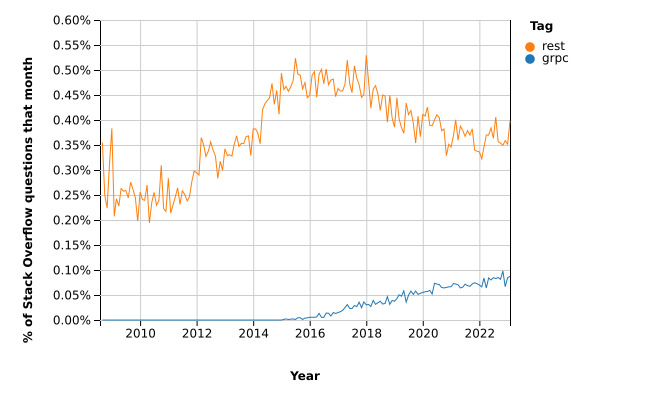
\includegraphics[width=1.0\linewidth]{stackoverflowgrpcrest}
    \caption{Percentage Stack Overflow vragen per maand voor gRPC en REST,\newline
    https://insights.stackoverflow.com/trends?tags=grpc\%2Crest}
    \label{fig:stackoverflowgrpcrest}
\end{figure}\\
\nocite{stackoverflowRESTgRPC}

Tot slot is het ook interessant om deze laatste grafiek in figuur~\ref{fig:stackoverflowRESTgRPCSOAPGraphQL} nog eens te bekijken, ditmaal echter met alle eerder genoemde API vari\"eteiten.

\begin{figure}[ht]
    \centering
    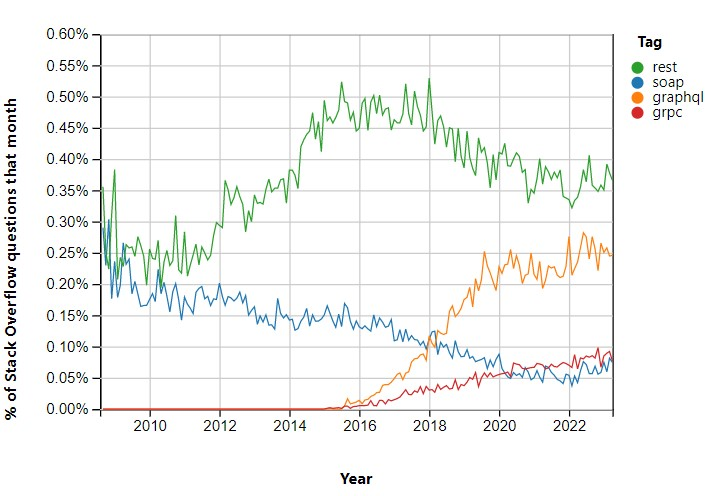
\includegraphics[width=1.0\linewidth]{stackoverflowRESTgRPCSOAPGraphQL}
    \caption{Percentage Stack Overflow vragen per maand voor REST, SOAP GraphQL en gRPC,\newline
    https://insights.stackoverflow.com/trends?tags=grpc\%2Crest}
    \label{fig:stackoverflowRESTgRPCSOAPGraphQL}
\end{figure}
\nocite{stackoverflowRESTgRPCSOAPGraphQL}

%XML vs JSON
